%!TEX root = ../main.tex
This chapter concerns the construction of the ACO framework. We will first discover how the framework is built and why. Then we will discover the choices of implementation and why they have been made. Finally, a complete explanation on how to use the framework is given with some examples that are used in chapter \ref{tests} for the tests.

\section{Analysis of the Implementations}\label{analysis}
There are many similarities and differences that can be identified in the different implementations discovered in chapter \ref{abstraction}. In this section, these common characteristics as well as the differences will be explained and developed. These observations will help to understand how the framework is built.

\subsection {Common characteristics}\label{common}

A first point that is common to the different implementations of chapter \ref{abstraction} is the use of the imput file. Each time, an input file containing information about the different cities is used. This information relates to the coordinates of the cities, the demand of a client in a CVRP case or the time windows for a VRPTW. This information can be easily parsed if it is normalized. \textbf{The reading of the input file} is thus considered as a first point that will be implemented in the framework.
 
Another common point is the way in which the \textbf{constraints that concern each client} are handled. As an example, for the CVRP, the demands of all clients are obviously associated with each client. The same goes for the Time windows in the VRPTW. Every time a constraint that concerns each client is added, that constraint is linked to the client. This link can be done in a generic way.

Another common point is the way of \textbf{representing the problem}. As explained in chapter \ref{introduction}, the problem representation for the TSP, CVRP and VRPTW is based on a graph. In all cases, the graph contains information about the cost (in time or length) to go from one city to another. Also, as explained in section \ref{whatisACO}, the ants uses stygmergy to communicate. \textbf{The representation of the pheromones} is also made using a graph. Indeed the pheromones are dropped on the arcs between the different cities.

Last but not least, the \textbf{construction algorithm} is very similar from one implementation to another. The core method used by the ant to build a path and the method that coordinates all the ants are the same in the application of the CVRP and the TSP. For the MACS-VRPTW, that is a more complicated implementation (see section \ref{applivrptw}), these methods are slightly different but there are still some similarities that are exploited in the framework.


\subsection{Differences}\label{differences}
 
In the implementation developed in sections \ref{applitsp}, \ref{applicvrp} and \ref{applivrptw}, some differences have been pointed out. For example, when the capacity constraints are added with the CVRP, some aspects have to be modified from the TSP to have a working algorithm. 

First, the capacity constraints that are added require that an ant keeps in memory her current load and the maximum load she can get. To do this, we need to create new variables for the ant. 

Then, the method to choose the next node must also be modified because of the capacity constraint. Indeed, an ant can not go to every city $j$ if she is at city $i$. Some cities will lead to a violation of the capacity constraint and thus can not be chosen. 

Next, the way the pheromones are updated on a path is different from one problem to another. This also leads to different implementations.

Finally, all the methods that permit to initialize or reset a path are slightly different in all the implementations because of the points listed above.

%%Expliquer la constructions des classes et objets et methodes qui vont implementer les points relevés au chapitre précédent. %%
\section{Architecture of the Framework}

From section \ref{analysis}, we can see that two big elements change with the problem and the constraints of the problem. This is the behavior of an ant and the synchronization between them via the pheromones. This is why two base classes that will handle these two behaviors are created. These two base classes will be extended by a user of the framework so that it has the desired behavior. 
The rest of the methods and information useful for the ACO application that we presented in section \ref{common} will be held in four different other classes that do not need to be modified, whatever constraints or changes are made to a VRP. In the figure \ref{fig:UML}, is the architecture of the framework described with an UML diagram. First, the four classes that will be constants in all the different possible implementations using the ACO framework are described: \texttt{VehicleRouting}, \texttt{FileReader}, \texttt{Graph} and \texttt{Client}. Then, the two classes that need to be extended by a user of the framework are described: \texttt{Ant} and \texttt{Colony}.
%\begin{landscape}
\begin{figure}
	\centering
		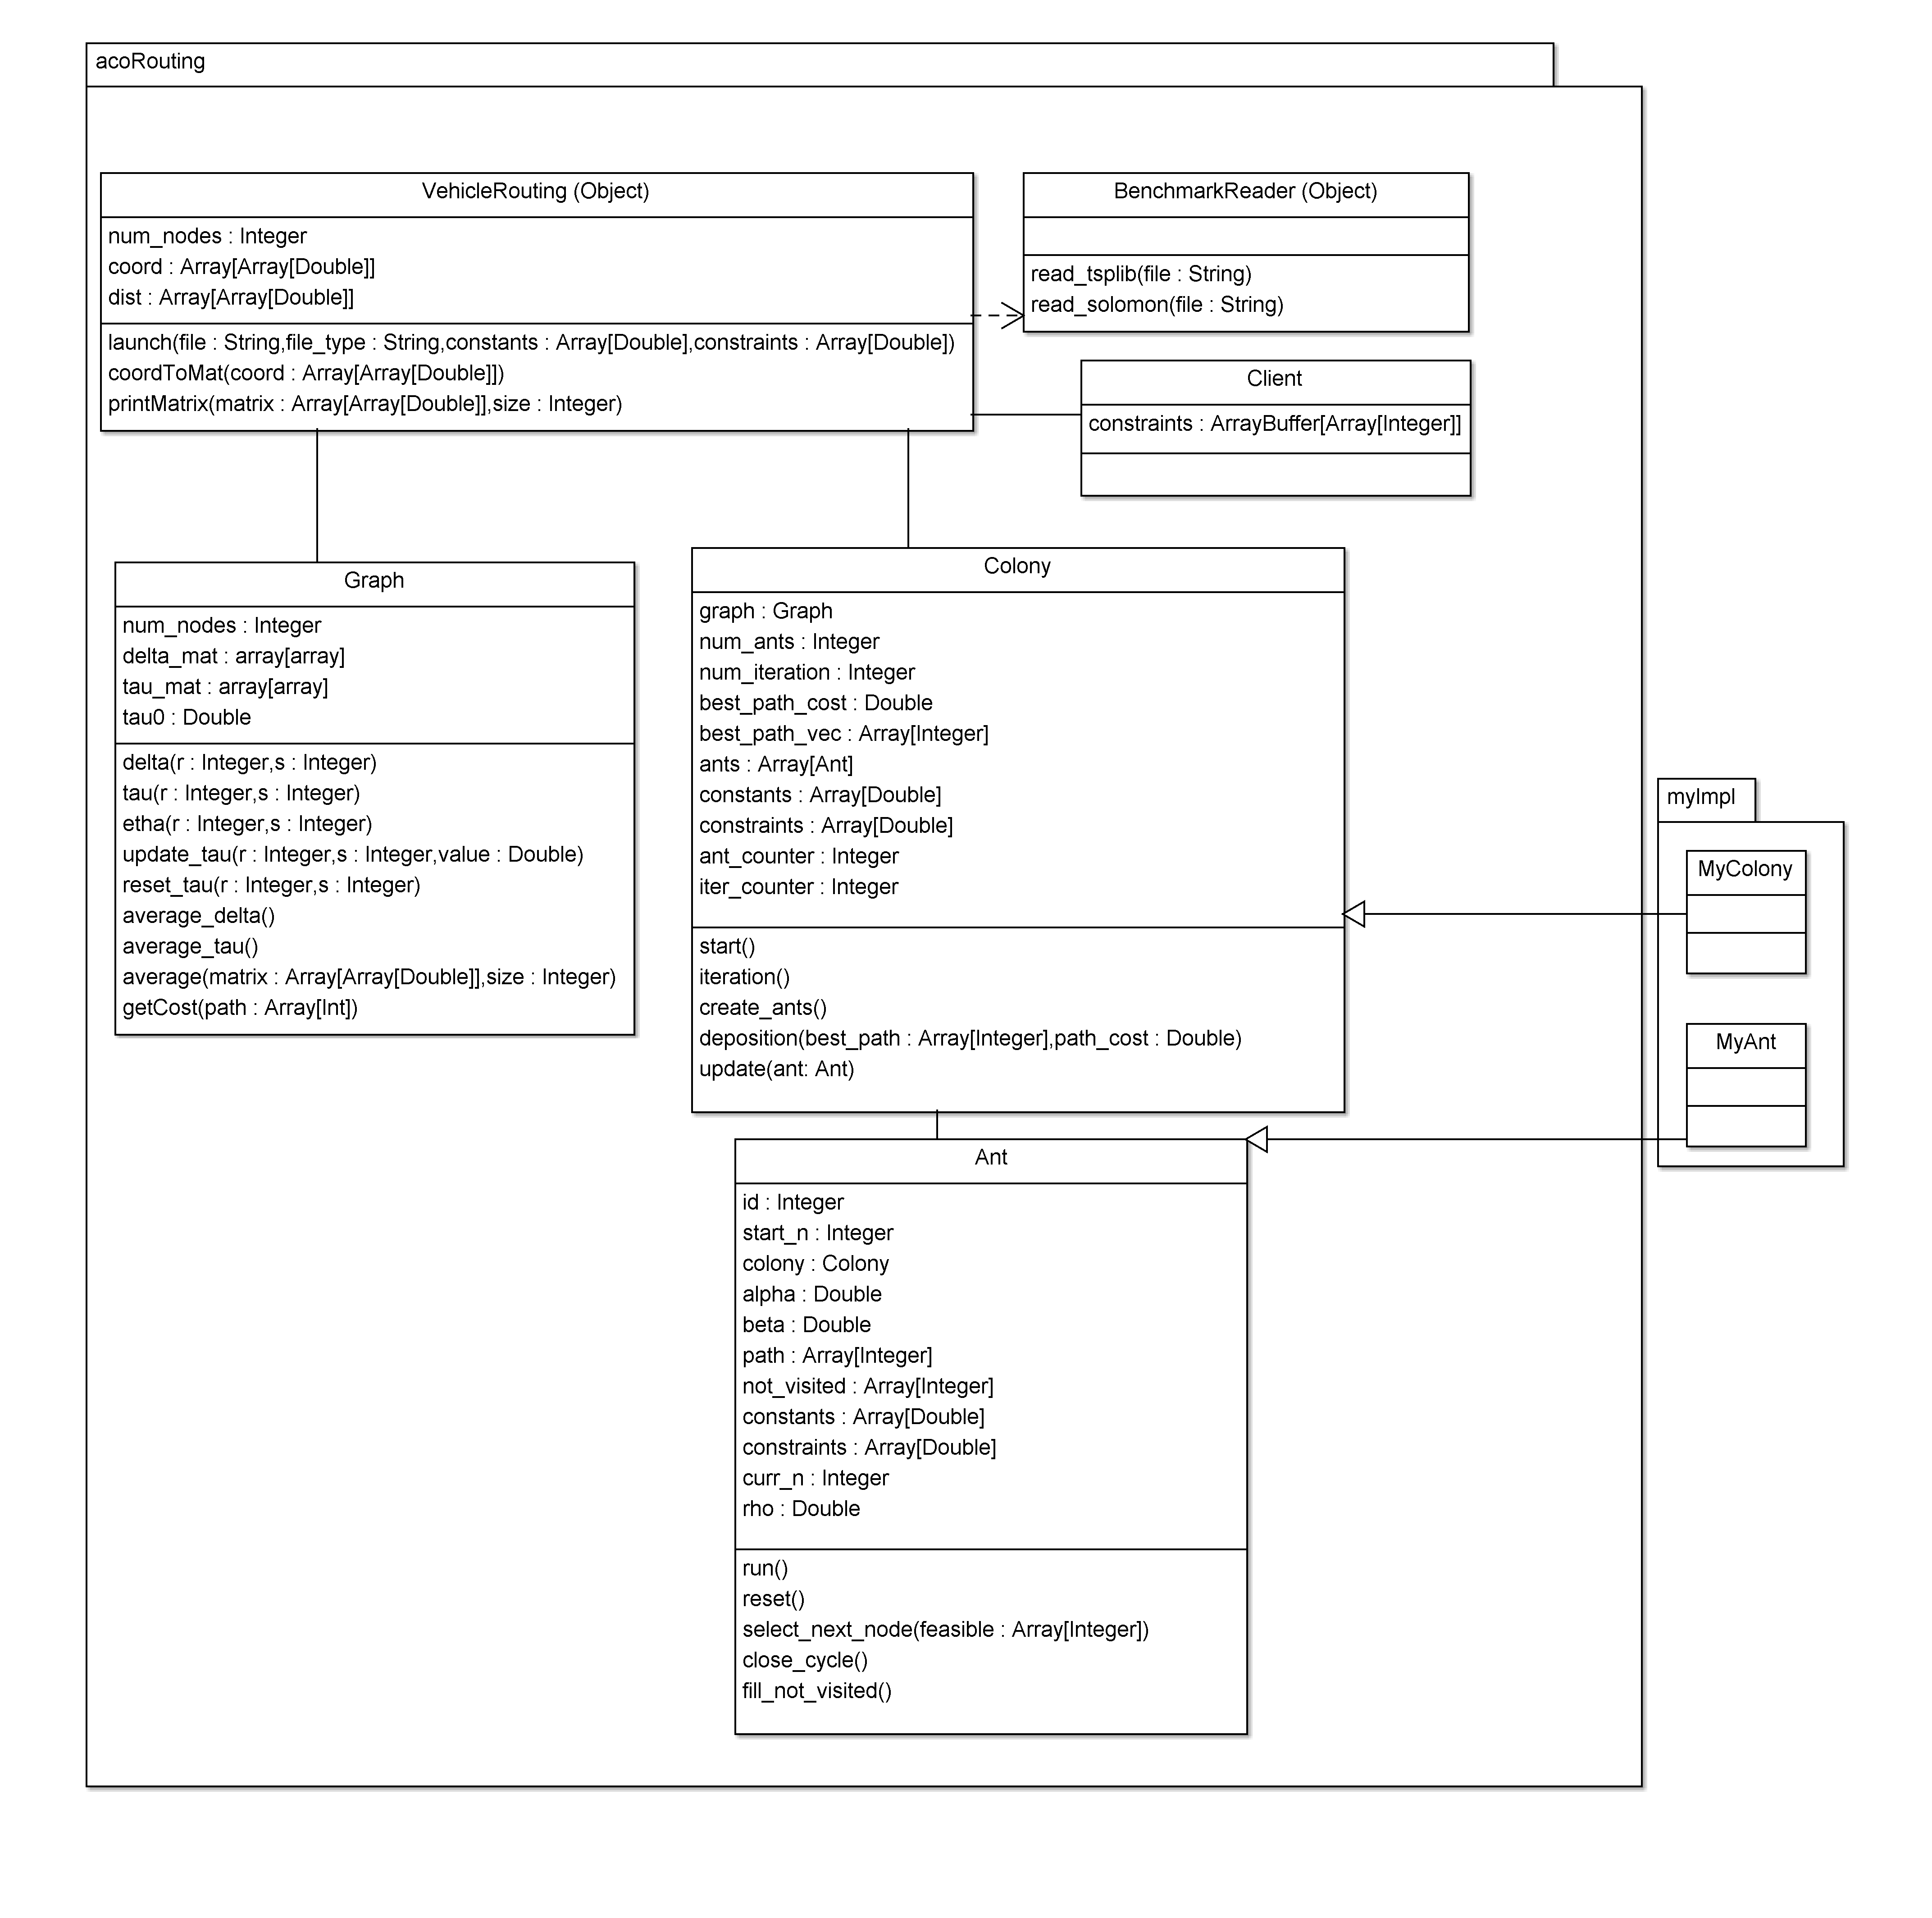
\includegraphics[scale = 0.1]{images/uml.png}
	\caption{UML diagram of the Framework developed.}
	\label{fig:UML}
\end{figure}
%\end{landscape}

\subsection{VehicleRouting object}\label{vrobject}
\begin{figure}
	\centering
		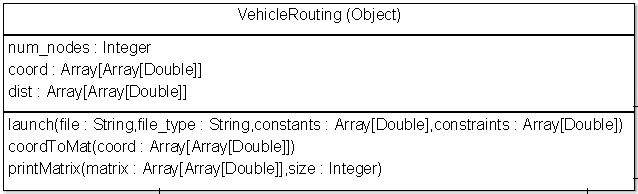
\includegraphics[scale = 0.5]{images/vehiclerouting.png}
	\caption{UML diagram of the VehicleRouting object.}
	\label{fig:vehiclerouting}
\end{figure}
The figure \ref{fig:vehiclerouting} is an UML representation of that object. This object is the "main" object of the framework.  It contains a method \texttt{launch(file:String,...)} that has for purpose of coordinating all the work done by the other classes. It uses the \texttt{FileReader} object methods to read the input file \texttt{file}. Then it transforms the data read into a matrix that will be used to create an instance of the Graph class. Finally it creates an instance of the \texttt{MyColony} class that will be used to find a solution to the problem. The method \texttt{coordToMat()} is used to transform the information contained in the input file that are cartesian coordinates into a distance matrix. A distance matrix is a square matrix $M$ that contains the distance between the city $i$ and $j$ at $M_{ij}$. The parameters of  the launch method are used to fix the number of iterations, the number of ants and other constants that are used in the program.

\subsection{BenchmarkReader object}
\begin{figure}
	\centering
		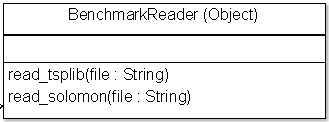
\includegraphics[scale = 0.5]{images/benchmarkreader.png}
	\caption{UML diagram of the BenchmarkReader object.}
	\label{fig:benchmarkreader}
\end{figure}
\texttt{BenchmarkReader} is an object that contains two methods \texttt{read\_tsplib(file)} and \texttt{read\_solomon(file)}. Each method can read a TSPLib file or a SolomonLib file respectively. The way a TSPLib file or SolomonLib file should be encoded is explained in section \ref{howtoframework}. The figure \ref{fig:benchmarkreader} is the representation of that object.

\subsection{Graph class}
\begin{figure}
	\centering
		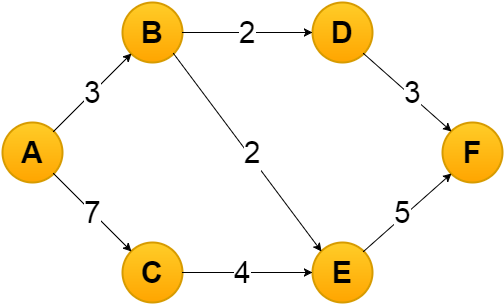
\includegraphics[scale = 0.5]{images/graph.png}
	\caption{UML diagram of the Graph class.}
	\label{fig:graph}
\end{figure}
Graph is a class containing all the information about the graph that represents the problem. This information is stored into the \texttt{delta\_mat} matrix. A Graph object is created by the VehicleRouting object after the input file has been read.
The graph class also contains information about the pheromones because they are held in a similar matrix, \texttt{tau\_mat}. The methods defined in the Graph class are used to access and modify these matrices.

\subsection{Client object}
\begin{figure}
	\centering
		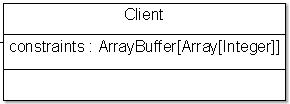
\includegraphics[scale = 0.5]{images/client.png}
	\caption{UML diagram of the Client object.}
	\label{fig:client}
\end{figure}
Client is a data object containing an ArrayBuffer \texttt{constraints} whose goal is to keep all the clients demands and constraints in that single array. The UML representation is in figure \ref{fig:client}.

\subsection{Colony class}
\begin{figure}
	\centering
		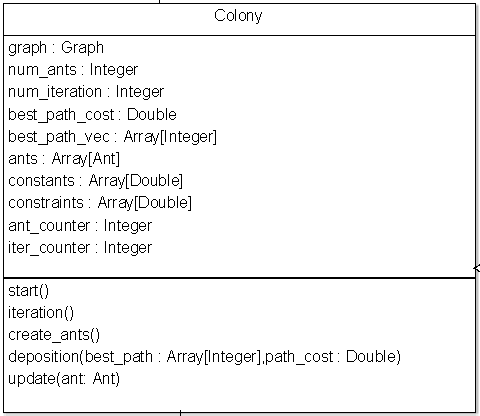
\includegraphics[scale = 0.5]{images/colony.png}
	\caption{UML diagram of the Colony class.}
	\label{fig:colony}
\end{figure}
The class Colony is an important class because it is the class that coordinates all of the ants that are used to solve a problem. The method \texttt{start()} creates all the ants that populate the colony (each ant is an instance of the \texttt{MyAnt class}). Then a loop that runs the ants is done until we reach a maximum fixed number of iterations. In that loop the method \texttt{iteration()} is called. This method runs each ant created using the \texttt{run()} method of these ants. When all ants have built their path, their results are compared and pheromones are dropped using the \texttt{deposition()} method. Finally, the best path is given to the \texttt{VehicleRouting} object that will print it.

\subsection{Ant class}
\begin{figure}
	\centering
	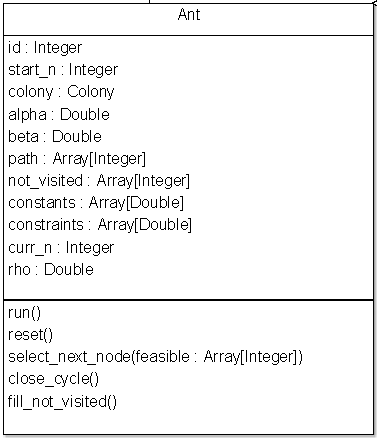
\includegraphics[scale = 0.5]{images/ant.png}
	\caption{UML diagram of the Ant class.}
	\label{fig:ant}
\end{figure}
The Ant class is also an important one because it is the class that controls the behavior of the ant. The core method of this class is the \texttt{run()} method. This method aims to make a path that is a solution to the problem. It will visit the cities one after another until there is no more city to visit. The choice of the next city to visit is made using the \texttt{select\_next\_node()} method. 

\subsection{MyColony - MyAnt}
These classes are intended to the user of the framework. These classes inherit from the \texttt{Colony} and \texttt{Ant} class respectively. The explanations about the way of completing these classes will be given in the next section (section \ref{howtoframework}).

%%%Explication sur les choix d'implémentation tels que le langage utilisé, les représentation des differentes structures de données etc etc.%%
\section{Implementation Choices}
In these sections the choices made for the implementation of the framework are explained. This covers the language used, the representation of the graph, the representation of the clients and the constraints associated to them, the parameters given to the different methods and the base case of the Framework.

\subsection{Language used}
The Scala language was carefully chosen. Scala is high level and a mixed paradigm language, it uses pure object-oriented and functional programming. The fact that it is object oriented allows for the creation of a framework that will be extended by inheritance by the user.

\subsection{Representation of the graph}
In routing problems, we always work with weighted graphs, graphs that have values attached to the edges. These values represent the cost of traveling from one node to the next. When we work with ACO, each ant has to access these values quite frequently. The weighted graph is thus represented as a weighted adjacency matrix. This choice permits to have access to the different value with a $O(1)$ complexity.

Let $v_i$ and $v_j$ be numbered vertices for $1\leq i,j\leq n$. Let $w_{ij}$ be the weight of an edge $e$ and assume that all edge weights are positive ($w_{ij}\geq 0$). Let $M[i,j]$ be an adjacency matrix where $M[i,j] = w_{ij}$ for each edge $e=(v_i,v_j)$. For each vertex $i$ in the graph, $M[i,i]=0$. 

Figure \ref{fig:adjacencymatrix} shows an example of a graph with its matrix representation.

\begin{figure}
	\centering
		\begin{subfigure}[b]{0.3\textwidth}
			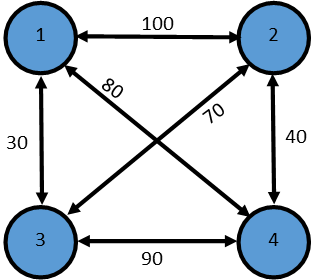
\includegraphics[width=\textwidth]{images/graph1.png}
			\caption{A simple weighted Graph}
		\end{subfigure}
		\qquad
		\begin{subfigure}[b]{0.3\textwidth}
			\begin{tabular}{cccc}
				0 & 100 & 30 & 80\\
				100 & 0 & 70 & 40 \\
				30 & 70 & 0 & 90 \\
				80 & 40 & 90 & 0 \\
			\end{tabular}
			\caption{Weighted adjacency matrix}
		\end{subfigure}
	\caption{A simple graph with its matrix representation}
	\label{fig:adjacencymatrix}
\end{figure}

\subsection{Client constraints}
	To represent the clients and the constraints associated to them, there are two choices: creating a Client class where each client is an instance of that class or creating a single Client object that contains all the information about all the clients of the problem in a single array. Because of the input file that presents the constraints in a sort of array, and because of the fact that an element in an array is accessed in $O(1)$, the second option is chosen.
		
	In the framework, a client Object is used, this object contains an ArrayBuffer named \texttt{constraints}. This ArrayBuffer contains an array for each constraints on the clients. For example, with a VRPTW of size $n$ (i.e.: with $n-1$ clients and 1 depot) the arraybuffer \texttt{constraints} is represented in figure \ref{fig:arraybuffer}. $Q_i$ represents the demand of client $i$. $a_i$ and $b_i$ represent respectively the begining and the end of the time window of the client $i$. If another constraint is added, a new array is added to the ArrayBuffer.
	\begin{figure}%
	\center
	\begin{tabular}{|c|c|c|}
		\hline
		\multicolumn{3}{|c|}{constraints} \\
		\hline
		0 & 1 & 2 \\
		\hline
		$Q_0$ & $a_0$ & $b_0$ \\
		$Q_1$ & $a_1$ & $b_1$ \\
		... & ... & ...\\
		$Q_n$ & $a_n$ & $b_n$ \\
		\hline
	\end{tabular}
	\caption{An example of the constraints arraybuffer}%
	\label{fig:arraybuffer}%
	\end{figure}
	
\subsection{Parameters of the launch method}\label{param}
	As explained in section \ref{vrobject}, the launch method has different parameters. The first is the location of the input file \texttt{file}. Then a string \texttt{file\_type} that says wich type of file is given in parameter (i.e.: Solomon or TSPLIB). The third and fourth are two arrays named \texttt{constants} and \texttt{constraints}. These arrays, as their names indicates, will contain the values of the constants used by the programs and the values associated to the constraints.
	
	The choice of an array to keep these values is made because it is flexible. If the user of the framework needs to use constants, he just has to pass an array that defines these constants. The same goes for the constraints. These two arrays are passed to the Colony and Ant instances. This also permits to the user to make a program that takes these arrays as parameters, so it is easy to manipulate and modify these constants.
	
	The \texttt{constants} array has a fixed minimum size. Some values, such as the number of ants to be used and the maximum number of iterations, must be the first two in the array. See figure \ref{tab:constants} for an example of the \texttt{constants} array.
	
	\begin{table}%
	\centering
	\begin{tabular}{|c|c|c|c|c|}
	\hline
	\# Ants & \# Iterations & $\alpha$ & $\beta$ & ...\\
	\hline
	\end{tabular}
	\caption{Representation of the \texttt{constants} array.}
	\label{tab:constants}
	\end{table}
	
	The \texttt{constraints} array is an array that is used by the ants to fix the limits that are given on the constraints. For example, in a CVRP, the ants (i.e. the trucks) have a maximum capacity limit. This limit is given in the constraints tabular. If other constraints of the same type must be added, this array is extended.
	
\subsection{Colony and Ant class}
	The ants that build solutions share common information, the pheromone matrix. This matrix is modified by the ants when they use an arc, and also when they all have completed a tour. This is where the colony class is important. The colony class collects the information about all the tours that the ants built, compares them and updates the pheromones using the best solution built by the ants.
	These two classes are also the base classes that will be extended by an user of the framework. The question is what contains these classes? 
	To answer that, we can make a first observation : The CVRP and the VRPTW are two generalizations of the TSP. Indeed, a TSP is a CVRP that has one vehicle with no capacity limit and customer with no demand. The same goes for the VRPTW, a TSP is a VRPTW with one vehicle, no capacity limit, no time limit and customer with no demand and infinite time-windows. 
	This observation leads to the implementation of the base problem (the TSP) in the base classes. This permits a user to directly use the framework without coding anything on a TSP problem. 
	In these classes can be found the methods that apply the base algorithm of an ACO system. These methods should not (or rarely) be modified. This is the \texttt{start()} and \texttt{iteration()} methods of the colony that are presented in the code block \ref{code:start} and the \texttt{run()} method of the ant presented in the code block \ref{code:run}. 
	
	\subsubsection{Colony}
	
	\begin{lstlisting}[captionpos=b, caption = Source code of the start and iteration method in Colony class, label= code:start]
def start() {
  this.create_ants
  while (!this.done) {
    this.iteration()
  } 
}

def iteration() {
  this.ant_counter = 0
  this.iter_counter += 1
  for (i <- 0 to num_ants - 1) {
    ants(i).run
  }
  this.deposition(this.best_path_vec, this.best_path_cost)
  if (this.best_path_cost < VehicleRouting.best_cost){
    VehicleRouting.best_tour = this.best_path_vec
    VehicleRouting.best_cost = this.best_path_cost
  }
  this.best_path_vec = Array(0)
  this.best_path_cost = Double.MaxValue
}
\end{lstlisting}
This fraction of code is a scala implementation of the ACO algorithm given in algorithm \ref{alg:acometa}. The Colony starts by creating the artificial ants. Then each ant is launched and does its work. When all the ants have made their tour, the best tour is used to drop pheromone with the \texttt{this.deposition()} method. If the best path found during this iteration is better than the best path found at the moment, it is replaced.


\subsubsection{Ant}
	
\begin{lstlisting}[captionpos=b, caption = Source code of the run method in Ant class, label= code:run]	
def run() {
  var new_node = 0
  while (this.not_visited.length != 0) {
    new_node = this.select_next_node(this.not_visited, null)
    this.path_cost += graph.delta(this.curr_n, new_node)
    this.path = this.path :+ new_node
    (this.graph.update_tau(curr_n, new_node, (1 - this.rho) 
		   * this.graph.tau(curr_n, new_node) 
			   + (this.rho * this.graph.tau0)))
    this.curr_n = new_node
  }
  close_cycle()


  this.colony.update(this)
  this.reset
}
\end{lstlisting}

The fraction of code presented in code block \ref{code:run} is the core method of the Ant. The \texttt{run()} method goal is to build a path that is a solution to the problem. The method iterates while the \texttt{not\_visited()} array is not empty. At each iteration:
\begin{itemize}
	\item a new node is selected
	\item the node is added to the path
	\item a local pheromone update is done according to equation \ref{eq:localpheromone}.
	\item the current node is replaced by the new selected node.
\end{itemize} 
When the iteration is done, the cycle is closed (the salesman goes back to his start point) and the results are sent to the Colony.


\section{How to use the framework}\label{howtoframework}
Now that we have a clear idea of the design of the framework, we will discover the convention governing its proper use. To do that, the correct way to use the framework to solve a CVRP problem will be elaborated. Some aspects change from the TSP base implementation of the framework. A capacity constraint is added. The Input file, the Client class and obviously the Colony and Ant classes change. The modifications are explained hereafter. 

\subsection{Input File}
The input file describing the problem must follow the convention of the TSPLIB file or the convention of the Solomon benchmark.
\subsubsection{TSPLIB}
The TSPLIB input file contains two part : a \emph{specification part} containing information on the file format and its content, and a \emph{data part} containing explicit data as the distances between cities. \cite{tsplib}
\paragraph{The specification part} contains :
\begin{itemize}
	\item the \emph{name} of the file.
	\item the \emph{type} of problem it describes (TSP, CVRP,...).
	\item the \emph{dimension} of the problem (Total number of nodes and depot in the case of a CVRP).
	\item the \emph{capacity} that specifies the truck capacity in a CVRP.
	\item the other constraints that can be added and their limitation on a truck.
	\item the \emph{edge weight type} that specifies how the distances are given.
\end{itemize}
\paragraph{The Data part} contains : 
\begin{itemize}
	\item the \emph{node\_coord\_section} where node coordinates are given in the form:
	\begin{verbatim}
	<integer> <real> <real>
	\end{verbatim}
	\item the \emph{depot\_section} that contains the list of depot nodes (always node 0 in our case)
	\item the \emph{demand\_section} that contains the demands of all nodes of a CVRP. It is given in the form: 
	\begin{verbatim}
	<integer><integer>
	\end{verbatim}
	\item the other constraints per node.
\end{itemize}

\subsubsection{Solomon Benchmark file}
The Solomon benchmark takes the form of a matrix. Each row contains all the information about a node. Table \ref{tab:Solomon} demonstrates the contents of the rows of that matrix.

\begin{table}%
\centering
\tiny
\begin{tabular}{l|l|l|l|l|l|l|l}
Client\_Number & X\_coordinate & Y\_coordinate & Demand & Ready\_Time & Due\_Date & Service\_Time & ... \\
\end{tabular}
\caption{A row of a Solomon benchmark file}
\label{tab:Solomon}
\end{table}
More columns can be added if there are more constraints to represent.
\cite{solomon}

\subsection{Constraints}
The CVRP is a TSP augmented with capacity constraints on the vehicle and demand of the client. In this section, we discover how to adapt the framework to solve the CVRP problem.
 
\subsubsection{Modelization of the constraints}
As outlined above, the CVRP adds one constraint to the TSP. It is the constraint bound to the capacity of the vehicle. 
The first change to make is of course in the input file. As explained before, a new set of data is added for each client: the demand.
The next changes we have to do are in the implementation of the Colony and the Ant. To do that, the class \texttt{MyAnt} and \texttt{MyColony} that \textbf{extends} the \texttt{Ant} and \texttt{Colony} class have to be implemented. 
\paragraph{The MyColony} class does not need many new methods. As the Ants do not start from a random city like in the TSP, but rather from the depot, the method \texttt{create\_ants()} is modified. The code of the \texttt{MyColony} class is presented in code block : \ref{code:colonycvrp}.

\begin{lstlisting}[captionpos=b, caption = MyColony implementation for a CVRP, label= code:colonycvrp]
class MyColony(graphp: Graph, num_antsp: Int, num_iterationp: Int) 
       extends Colony(graphp, num_antsp, num_iterationp) {

  override def create_ants() {
    var startcity = 0
    this.ants = Array.empty[MyAnt]
    for (i <- 0 to (num_ants - 1)) {
        startcity = 0
    var ant = new MyAnt(i, startcity, this, VehicleRouting.capacity)
        ants = ants :+ ant
    }
    ants
  }
}
\end{lstlisting}
\paragraph{The MyAnt} class needs more modifications. The capacity constraint has to be taken into account when selecting the next node. To do that, different methods are possible. The simplest is to follow the selection process as for the TSP and send the truck back to the depot if the selected node violates the constraints. In that case, only the \texttt{select\_next\_node()} method must be overridden. Below is the new implementation of the \texttt{select\_next\_node()} method.
\begin{lstlisting}[captionpos=b, caption = MyAnt implementation for a CVRP, label= code:antcvrp]
override def select_next_node(feasable: Array[Int]): Int = {
    val graph = this.graph
    var new_node = -1
    var denominator = 0.0

    if (feasable(0) == 0) { 
      return 0
    }
    if (!feasable.isEmpty) {
      denominator = compute_denominator(feasable)
      new_node = choose_new_node(denominator, feasable)
      if (new_node == -1) {
        new_node = this.curr_n
      }
      if (this.capacity < Client.constraints(0)(new_node) + this.load) {
        new_node = 0
        this.load = 0
      } else {
        this.load += Client.constraints(0)(new_node)
        this.not_visited = this.not_visited.filterNot(_ == new_node)
      }
      return new_node
    } else {
      new_node = 0
      this.load = 0
      return new_node
    }
  }
\end{lstlisting}

\subsection{Adding new Constraints}
In this section, through two other examples, it is shown how to add other constraints to a CVRP. The two examples that are described in this section will be tested in chapter \ref{tests}. 

The first example concerns the adding of a constraint to a CVRP that is verified after a tour is built. In other words, an ant constructs a valid path according to the capacity constraint. This path must then be validated to be sure it does not violate other constraints. This type of constraint is used in some vehicle routing problems with black box feasibility (3D loading ...) \cite{massen2013vrp}. This type of constraint is called "off-parcour constraint".

The second example concerns the adding of a soft constraint that is used in the construction of a tour. We talk about a soft constraint because the constraint will be used in the evaluation of the quality of a solution provided (i.e. in the objective function). A soft constraint can not be violated but must be taken into account in the building of a solution to have a correct solution. This type of constraint is called "in-parcour constraint".

The third example is a hard "in-parcour constraint". What is called a hard constraint is, as the capacity of a CVRP, a constraint that can not be violated.

\subsubsection{Off-parcour constraint}
	In this section is explained the adding of an off-parcour constraint. In this example, a simple rule is implemented but the case can be generalized to any more complex rules. In this example, the rule forbids two cities that have consecutive numbers to be visited one after the other. In other words, a city $i$ can not be visited after city $i-1$ or city $i+1$.
	
	To implement this rule, from the CVRP implementation given above, we only need to modify the \texttt{MyColony}. Indeed, the \texttt{MyAnt} class does not need modifications because the constraint that we add can not be verified in the path construction but only when the path is finished. 
	
	When an ant has finished building a path, the colony has to test whether or not the path is the shortest found in this iteration and whether or not the path is valid according to the rule we defined. This is done with both methods \texttt{update(ant:Ant)} and \texttt{is\_valid(ant:Ant)}. The code of these functions is given in code block \ref{code:offconstraint}.
	
	\begin{lstlisting}[captionpos=b, caption = Method used for the off-path constraints, label= code:offconstraint]
 override def update(ant:Ant){
    this.ant_counter += 1
    if(is_valid(ant)){
      if (ant.path_cost < this.best_path_cost) {
        this.best_path_cost = ant.path_cost
        this.best_path_vec = ant.path
      }
    }
  }  
  def is_valid(ant:Ant):Boolean={
    var last=0
    for(c <- ant.path ){
      if (last != 0){
        if(last+1 == c || last-1 == c){
          return false
        }
      }
      last=c
    }
    return true
  }\end{lstlisting}

The method \texttt{update(ant:Ant)} is called every time an ant has build a path. The update method checks first if the path is valid using the \texttt{is\_valid(ant:Ant)} then keeps the solution of the ant if it is the best of the iteration. If the path is not valid, it is discarded. In this case the method \texttt{is\_valid(ant:Ant)} is quite simple but it can be replaced by something different easily.

\subsubsection{In-parcour constraint}\label{inconstraints}
\paragraph{The soft constraint} that is implemented is a preference for the client to be placed first in a subtour. Each client has a value assigned to him that represents how important it is to be the first in a subtour. The value of that preference is an integer in the range $0$ through $10$, $10$ symbolizing a great need to be first and $0$ symbolizing the fact that a client does not want to be first.

To implement that constraint, the first thing to do is to add the preference of each client in the input file. Once this is done, the \texttt{MyAnt} class must be modified to take the constraint into account. A different random proportional rule will be used when the ant is at the depot (that is the city $i = 0$). Instead of using the classical one presented in equation \ref{eq:cvrp proportional rule}, when at city $i = 0$ a new factor is added to the equation to take into account the preferences of each client. The new rule that is used is :
\begin{equation}
	p_{0j}^k =
	\begin{cases}
		\frac{[\tau_{0j}]^\alpha [\eta_{0j}]^\beta [\xi_{j}]^\epsilon}{\sum_{l\in N_i^k}{[\tau_{0l}]^\alpha [\eta_{0l}]^\beta [\xi_{l}]^\epsilon}} & \text{if } j\in N_i^k\\
		0 & \text{otherwise}
	\end{cases}
\label{eq:modifproportionalrule}
\end{equation}
where $\xi_{j}$ is the value associated with client $j$ and $\epsilon$ is a constant as $\alpha$ and $\beta$ that affects the importance of $\xi$ in the building of a solution. As $\epsilon$ is a constant, the value of that constant is added into the array \texttt{constants} presented in section \ref{param}.

The second thing to change is the objective function that measures the quality of a tour in the \texttt{MyColony} class. To do that, instead of taking only the length of the path to give a cost to a solution, we add to that cost a value related to the preference of each first client in a subtour (see code block \ref{code:soft}).

\begin{lstlisting}[captionpos=b, caption = Taking the preference into account , label= code:soft]
  override def update(ant: Ant) {
    this.ant_counter += 1
    var first_in_tour = new ArrayBuffer[Int]
    var cost = ant.path_cost
    for (i <- 0 to ant.path.length-1){
      if(ant.path(i)==0){
        first_in_tour += ant.path(i+1)
      }
    }
    for (a<-first_in_tour){
      cost += ((math.abs(Client.constraints(1)(a)-10))*100)
    }
    if (cost < this.best_path_cost) {
      this.best_path_cost = cost
      this.best_path_vec = ant.path
    }
  }
	\end{lstlisting}
	
	Again this example is a simple one. The objective function and the proportional rule used are maybe not the best in that case, but the goal of this example is just to show how to add constraints and what it implies in the implementation.

\paragraph{The hard constraint} that is implemented here is a limit on a sub-path of a CVRP solution. As a reminder, a CVRP solution is a set of paths where each path begins and ends at the depot and visits some cities. To the classic CVRP that limits only the capacity of a vehicle, we add here a limit on the maximum length of a subpath. This limit can represent, for example, the size of the fuel tank of a truck. Adding that kind of constraint is done by modifying the ant behaviour. This is done in the implementation of the \texttt{MyAnt} class by overriding the \texttt{select\_next\_node(feasable:Array[Int])} method. In the implementation of the CVRP given above, we force the ant to go back to the depot if the next node selected in the path violate the constraint capacity. To take the new constraint into account, we simply need to calculate and keep in memory the length of the subtour, and send the truck back to the depot if the constraint is violated (if the subtour is too long).
In this example the \texttt{constraints} array that is defined as an argument in the \texttt{launch} method of the VehicleRouting object (see section \ref{param}) will contain a new value that will represent the maximum length of a tour.

